\onehalfspaced
\chapter{Quality Control for Crowdsourcing Machine Translation}
Quality control is an important issue for crowdsourcing annotation and labeling since workers in the crowdsourcing community are not required to provide the qualification to do the job. \newcite{sheng2008get}'s work on repeated labeling presents a way of solving the problems of uncertainty in labeling in crowdsourcing. Since we cannot always get high-quality labeled data samples with relatively low costs in reality, to keep the model trained on noisy labeled data having a high accuracy in predicting, \newcite{sheng2008get} proposed a framework for repeated-labeling that resolves the uncertainty in labeling via majority voting. The experimental results show that a model's predicting accuracy is improved even if labels in its training data are noisy and of imperfect quality.  As long as the integrated quality (the probability of the integrated labeling being correct) is higher than 0.5, repeated labeling benefits model training. 

To improve the quality of crowdsourcing machine translation, \cite{zaidan-callisonburch:2011:ACL-HLT2011a}  solicited four translations for each source sentences. By selecting the best translation among them, they achieved a professional level of quality compared to gold standard references. We extended their framework to other models.

\section{Data Collection}

We use the data collected by  \newcite{zaidan-callisonburch:2011:ACL-HLT2011a} through Amazon's Mechanical Turk(MTurk). MTurk is an online platform provided to people for completing Human Intelligence Tasks(HIT) with a relatively low cost. We use their Urdu-to-English 2009 NIST Evaluation Set as our corpus.  \newcite{zaidan-callisonburch:2011:ACL-HLT2011a}  translated the Urdu side to English through MTurk. They collected the translations in the unit of Human Intelligence Tasks(or HITs). In every HIT, they posted 10 Urdu sentences to be translated. Every sentence is translated by 4 workers, and subsequently post-edited by 10 additional workers.\footnote{\newcite{zaidan-callisonburch:2011:ACL-HLT2011a}  collected their translations in two batches.  The first batch contained 1 translation, each with 1 post-edited  version.  The second contained an additional 3 translations, each of which was post-edited by 3 workers.}
This data set also has four corresponding professional translations for each  of the Urdu sentences, collected by LDC. This makes it possible to compare the Turkers' translation quality to professionals.  
\section{Feature Extraction}
Following \newcite{zaidan-callisonburch:2011:ACL-HLT2011a}, we extract a number of features from the translations and workers' self-reported language skills.  We use these to build feature vectors used in tuning model and choosing the best translations from the candidates. 
POTENTIALLY: We extend \newcite{zaidan-callisonburch:2011:ACL-HLT2011a}'s feature set to include additional bilingual features, which were not part of that original work.
\subsection{Sentence-Level Features (9 Features)}
This feature set contains language based features to solely implicate the quality of an English sentence without any suggestion on the bond of the meaning between the source sentence and the translation . This set of features tells good English sentences apart bad ones. The reason we use this set of features is that a good English sentence is the prerequisite of being a good English translation.
\begin{itemize}
\item Language model features:	we assign a log probability and a per-word perplexity score for each sentence. We use SRILM toolkit to calculate perplexity score for each sentence based on 5-gram language model trained on English Gigaword corpus.
\item Sentence length features:	we use the ratio of the length of the Urdu source sentence to the length of  the translation sentence as feature since a good translation is expected to be comparable in length with source sentence. We add two such ratio features( one is designed for unreasonably short translation and the other is for unreasonably long translation).
\item Web \textit{n}-gram log probability feature: we add the Web \textit{n}-gram log probability feature to reflect  the probability of the \textit{n}-grams(up to length 5) exist in the Microsoft Web N-Gram Corpus. For short sentences whose length is less than 5, we use the sentence length as the order of the \textit{n}-gram in calculation.
\item Web \textit{n}-gram geometric average features: we calculate the geometric average \textit{n}-gram  to evaluate the average matching over different \textit{n}-grams. We add 3 features correspondent to max \textit{n}-gram length of 3,4 and 5. Specifically, $P_i$ denotes the log probability of \textit{i}-gram and these 3 features are represented in $\sqrt[3]{P_1 P_2 P_3}$ ,$\sqrt[4]{P_1 P_2 P_3 P_4}$ and $\sqrt[5]{P_1 P_2 P_3 P_4 P_5}$ .
\item Edit rate to other translations: In posterior methods, to minimize Bayes risk, we choose the translation  that is most similar to other translations. Taking this into consideration, we add the edit rate feature to implement the similarity among all candidates translations.
\end{itemize}
 \subsection{Worker-Level Features}
 We take the quality of workers into consideration and add worker level features since the intuition that good workers can always high quality translations.
\begin{itemize}
\item	Aggregate features:	for each sentence level feature, we use the average values over all translations provided by the same worker as that worker's aggregate feature values.
\item	Language abilities:	we collect worker's language ability information about whether the worker is a native Urdu speaker or native English speaker and how long they have spoken English or Urdu and add four features correspondent to the four aspects above.
\item	Worker Location:	we add two features to indicate whether a worker is located in Pakistan or India.
\end{itemize}
 \subsection{Ranking Features}
 \newcite{zaidan-callisonburch:2011:ACL-HLT2011a} collected 5 ranking labels for each translation and refine 3 features from these labels.
 \begin{itemize}
 \item Average Ranking:	the average of the 5 ranking labels for this translation.
 \item Is-Best percentage: this feature shows how often a translation is ranked as the best translation among all candidates translation.
 \item Is-Better percentage: how often a translation is ranked as a better translation based on the pairwise comparisons.
  \end{itemize}
 \subsection{Calibration Features}
 \begin{itemize}
 \item Calibration features: 1 feature based on the average BLEU score of a worker's translations provided is computed against professional references.
\end{itemize}

We additionally introduce a new bilingual feature based on IBM Model 1. We align words between each candidate translation and its corresponding source sentence. The bilingual feature for a translation is the average of its alignment probabilities. In Figure \ref{biexample1}, we show how the bilingual feature allows us to distinguish between a valid translation (top) and an invalid/spammy translation (bottom).

\begin{figure}[!htb]
  \centering
  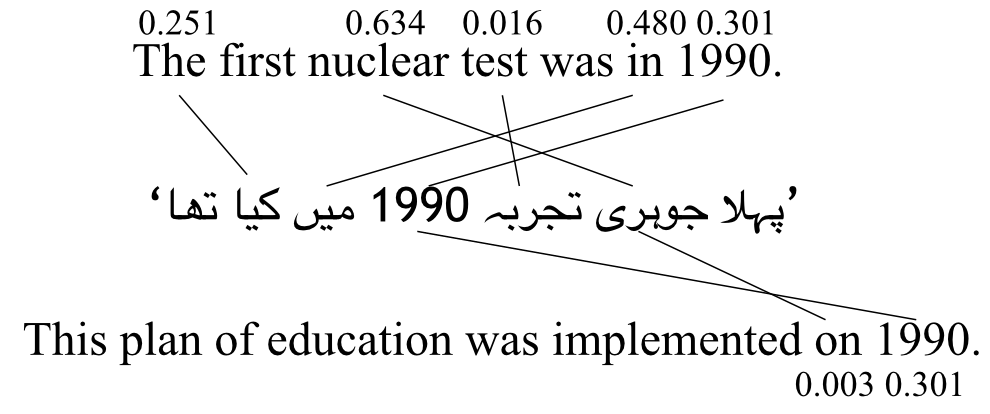
\includegraphics[width=0.7\textwidth]{bilingualexample/example.png}
  \caption{Example bilingual features for two crowdsourced translations of an Urdu sentence. The numbers are alignment probabilities for each aligned word. The bilingual feature is the average of these probabilities, thus 0.240 for the good translation and 0.043 for the bad translation. Some words are not aligned if potential word pairs don't exist in bilingual training corpus.
}
    \label{biexample1}
\end{figure}

\section{Supervised Learning in Machine Translation}
Supervised learning methods can be used to discriminate good translations and bad translations, and train models to estimate the quality of translations. \cite{zaidan-callisonburch:2011:ACL-HLT2011a} proposed a framework to select the best translation among all candidates and achieved professional translating quality. They used MERT as the parameter tuning model. We extended their framework by using decision tree model and linear regression model.

\subsection{MERT}

\newcite{och2003minimum} proposed the Minimum Error Rate Training (MERT) framework in statistical machine translation. This framework is used to train models to score each translation and discriminate good translations and bad translations. Since each translation candidate is represented in feature vector format, the model is just a set of parameters corresponding to each feature. Given the n-best list translations of each source sentence and their corresponding professional references, instead of searching the huge space for all parameters, they used Powell algorithm \cite{powellefficient} in the parameter tuning process where every time they only change the value of one parameter and detect the performance based on that value. 

Suppose the feature vector used to represent the translation candidate $x$ is defined as:\\
\begin{align}
H(x) = \{h_1(x),h_2(x),..,h_n(x)\}
\end{align}
and in the log-linear model, the overall translation probability (quality) is predicted as:
\begin{align}
p(x) = \exp\sum_{i=1}^{n}\lambda_ih_i(x)
\end{align}
where $\lambda_i$ is the parameter for the $i_{th}$ feature. In Powell Search, if we want to search for the best value of feature $h_c(x)$ in some iteration, then the probability of that translation could be represent as:
\begin{align}
p(x) =& \exp (\lambda_{c}h_c(x)+u(x))\\
u(x) =&\sum_{i \neq c} \lambda_i h_i(x)
\end{align}
Each translation is a line with a slope of $h_c(x)$ and an offset of $u(x)$ in a 2-dimensional space. Thus, for the n-best translation candidates, we have $n$ lines in the space and the top line means the corresponding translation has the highest model predicted probability. However, as the value of $\lambda_c$ changes, the top line may also change since there might be intersects among these lines. Thus, there exists several intervals for the value of $\lambda_c$ and for each interval, there is a particular top line which means when the value of $\lambda_c$ belongs to that interval, the corresponding translation has the highest model predicted score.  These intersects are called threshold points. 
For every value $v$ that could be assigned to $\lambda_c$, we could rank the n-best translations for each source sentence in the training set based on the metric of $p(x) = \exp (v\cdot h_c(x)+u(x))$, select the top translation for each source sentence and calculate the quality score for these translations against professional translations in some evaluation metric, such as BLEU. Our goal is to find the best value for $\lambda_c$ that results the highest quality score for those top translations we select for each source sentence. Even though we only search for the best value searching for the best value for a single parameter,it still costs lots of time, especially when the parameter could be in real numbers. However, we know that for each source sentence, the top line only changes at threshold points, which means we only have to search for the best value of $\lambda_c$ in a finite state set. Figure \ref{mert1} is the framework \cite{koehn2009statistical} for MERT to tune the parameter.
\begin{figure}[!htb]
  \centering
  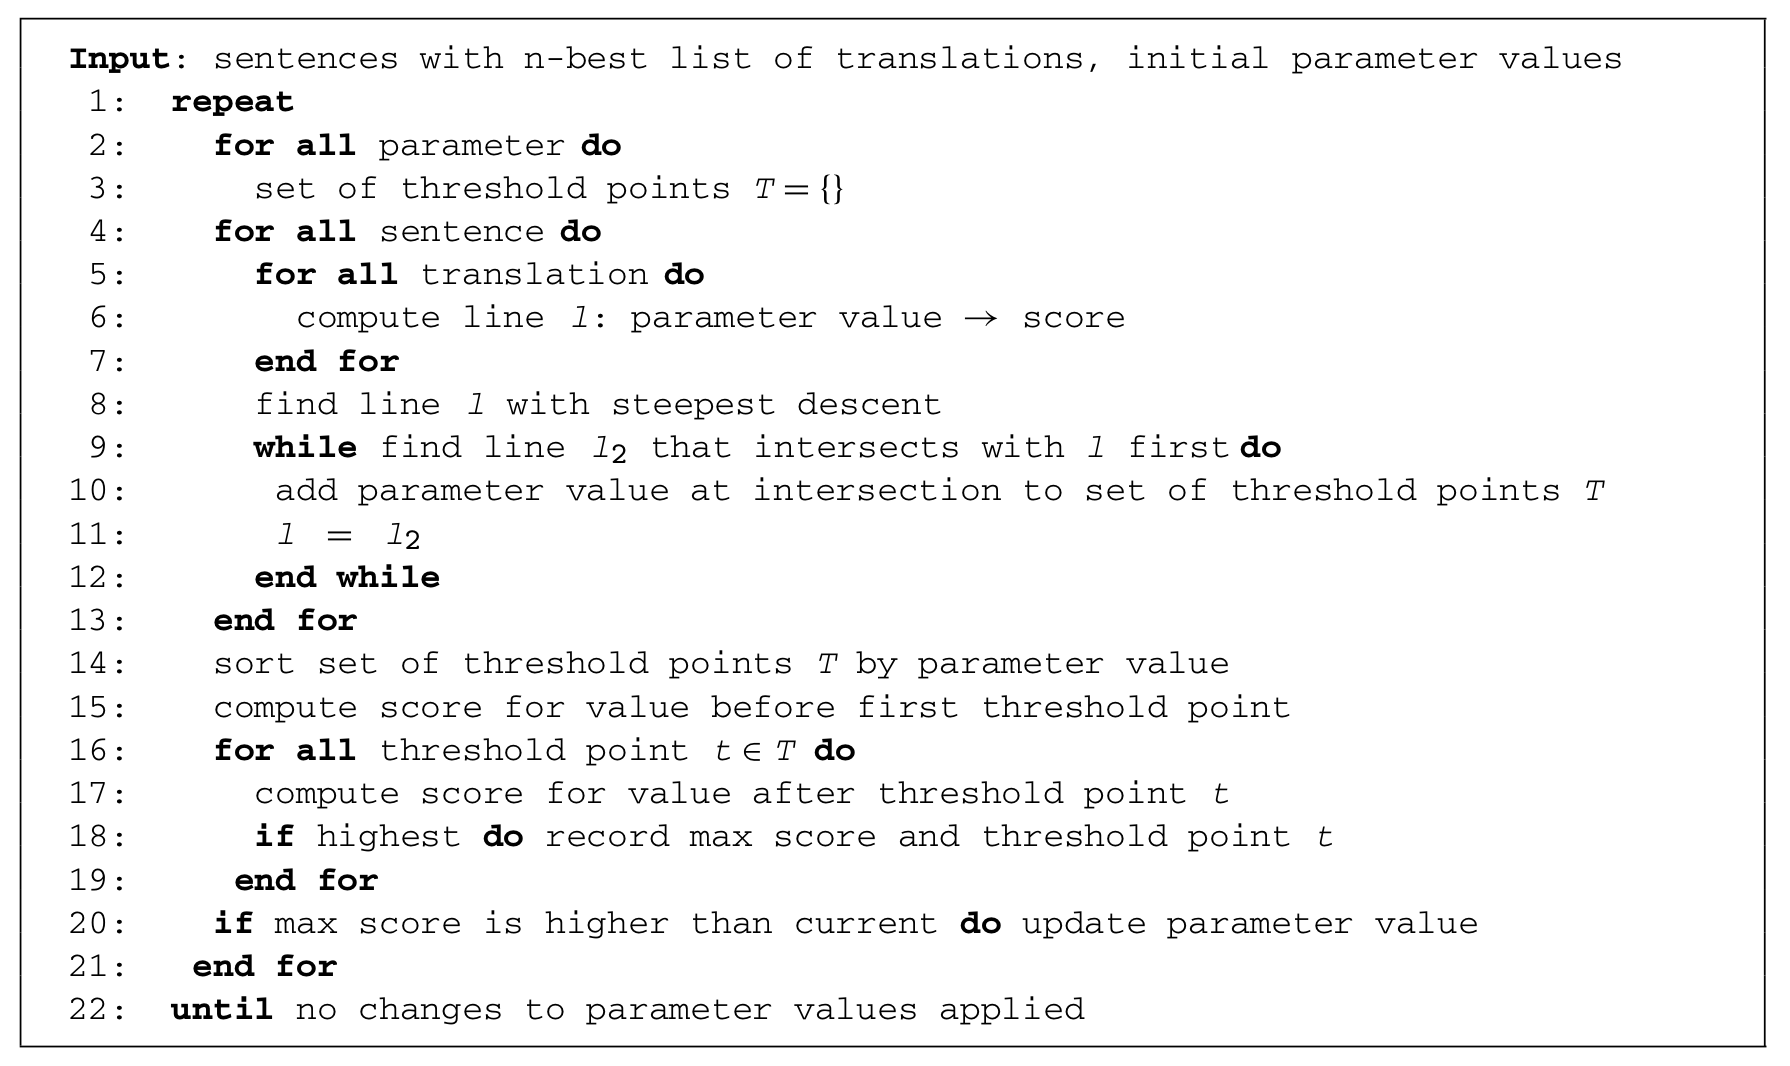
\includegraphics[width=0.7\textwidth]{MERT/mert.png}
  \caption{The Framework for the parameter tuning process using Powell search.
}
    \label{mert1}
\end{figure}

\subsection{Decision Tree}

Decision Tree is a classical machine learning model in classification and regression. In our case, we only introduce the regression tree, which is very similar to classification tree. The basic framework to train a regression tree is partition since we want to divide the data based on some attributes so that data in the same sub-division has similar property (label).  The framework to grow a decision tree is shown below:\\
1. Start with an empty tree.\\
2. If the stopping rule is not satisfied, make partition on next best feature selected by variance reduction.\\
3. Recursion on each leaf.\\
Variance reduction is a splitting criterion to evaluate the effectiveness of the best feature and the splitting threshold for that feature. At node $t$, we want to maximize the variance reduction $\Delta i(s,t)$ by choosing the best split $s$. $\Delta i(s,t)$ is defined as:
\begin{align}
\Delta i(s,t) =& i(t) - P_L i(t_L)-P_Ri(t_R)\\
\Delta i(t) = & \frac{\sum_{n \in h(t)} w_n f_n (y_n - \bar{y}(t))^2}{\sum_{n \in h(t)} w_n f_n}\\
P_L = & \frac{ N_w(t_L)}{N_w (t)}\\
P_R = & \frac{ N_w(t_R)}{N_w (t)}\\
N_w(t) = & \sum_{n \in h(t)} w_n f_n\\
\bar{y}(t) = & \frac{\sum_{n \in h(t)} w_n f_n y_n}{N_w (t)}
\end{align}
where $h(t)$ is the learning samples at node $t$,$w_n$ is the weight associated with sample n, $f_n$ is the frequency weight associated with sample n. The splitting process stops when a node becomes pure, all samples have the same set of input attributes, the variance reduction is less than some user set threshold and so on.

\subsection{Linear Regression}
Linear Regression is a linear model based on the goal to reduce the residual squared error. It's an approach to model the relationship between a scalar variable $y$ and the corresponding feature vector $x$. From a matrix perspective, given a set of feature matrix $X$ and its corresponding label vector $\vec{y}$, the model is $w = (X^{T}X)^{-1}X^{T}\vec{y}$. 

\section{Experiments}

We extended \cite{zaidan-callisonburch:2011:ACL-HLT2011a}'s framework using different models trained on different feature sets. We use 10\% of the whole data set as the training set and use the rest as the test set.  Each source sentence has four translations in total. We evaluate the translation quality in BLEU. We report results based on five-fold cross validation.
\subsection{Baseline}
Random selection is set as the baseline method which select a translation among all four translations randomly and achieves a BLEU score of 29.56. We also perform an Oracle experiment to select the best professional translation  among all four references by comparing one translation against other three translations and selecting the one with highest similarity to others. Oracle experiment achieves a BLEU score of 42.38.
\subsection{MERT}
We replicate \cite{zaidan-callisonburch:2011:ACL-HLT2011a}'s framework on MERT with the new added bilingual feature. Table \ref{mertbleu} shows the translation quality. 
\begin{table}[h]
\center
\begin{tabular}{c|c}
\hline
Feature Set           & BLEU Score \\ \hhline{==}
(S)entence features   & 38.51      \\ \hline
(W)orker features     & 37.89      \\ \hline
(R)anking features    & 36.74      \\ \hline
(C)alibration feature & 38.27      \\ \hline
S+W+R features        & 38.44      \\ \hline
S+W+R+B features      & 38.80      \\ \hline
All features          & 39.47      \\ \hline
\end{tabular}
\caption{The translation quality for MERT}
\label{mertbleu}
\end{table}
\subsection{Decision Tree}
We use the Decision Tree model to substitute the MERT model in the original framework. 
 Table \ref{dtbleu} shows translation quality. 
\begin{table}[h]
\center
\begin{tabular}{c|c}
\hline
Feature Set           & BLEU Score \\ \hhline{==}
(S)entence features   & 35.32      \\ \hline
(W)orker features     & 37.59      \\ \hline
(R)anking features    & 36.17     \\ \hline
(C)alibration feature & 38.27      \\ \hline
S+W+R features        & 37.04     \\ \hline
S+W+R+B features      & 37.00    \\ \hline
All features          & 37.19     \\ \hline
\end{tabular}
\caption{The translation quality for Decision Tree}
\label{dtbleu}
\end{table}
We visualize the decision tree we trained using all features. Figure \ref{dtexample} shows the visualization. In the visualization graph, label names is the shorten form of the feature names.
Table \ref{senfeatures}, Table \ref{workerfeatures},Table \ref{rankingfeatures},Table \ref{calibilinfeatures} show label names and their corresponding feature names.

\begin{table}[h]
\center
\begin{tabular}{cc}
\hline
\multicolumn{2}{c}{Sentence-Level Features}                              \\  \hhline{==}
\multicolumn{1}{c|}{LOGPROB}      & Sentence Log Probabilty              \\ \hline
\multicolumn{1}{c|}{AVGPPL}       & Per-Word Perplexity Score            \\ \hline
\multicolumn{1}{c|}{LengthRatio1} & Length Ratio Feature 1               \\ \hline
\multicolumn{1}{c|}{LengthRatio2} & Length Ratio Feature 2               \\ \hline
\multicolumn{1}{c|}{NGramMatch}   & Web N-Gram Log Probability Feature   \\ \hline
\multicolumn{1}{c|}{Root3}        & Web 3-Gram Geometric Average Feature \\ \hline
\multicolumn{1}{c|}{Root4}        & Web 4-Gram Geometric Average Feature \\ \hline
\multicolumn{1}{c|}{Root5}        & Web 5-Gram Geometric Average Feature \\ \hline
\multicolumn{1}{c|}{AvgTER}       & Edit Rate Feature                    \\ \hline
\end{tabular}
\label{senfeatures}
\caption{Labels for sentence-level features}
\end{table}
 
 \begin{table}[h]
 \center
\begin{tabular}{cc}
\hline
\multicolumn{2}{c}{Worker-Level Features}                                                          \\ \hhline{==}
\multicolumn{1}{c|}{AGLOGPROB}        & Workers' Aggregate Feature of Sentence Log Probabilty      \\ \hline
\multicolumn{1}{c|}{AGAVGPPL}         & Workers' Aggregate Feature of Per-Word Perplexity Score    \\ \hline
\multicolumn{1}{c|}{AGLengthRatio1}   & Workers' Aggregate Feature of Length Ratio 1               \\ \hline
\multicolumn{1}{c|}{AGLengthRatio2}   & Workers' Aggregate Feature of Length Ratio 2               \\ \hline
\multicolumn{1}{c|}{AGNGramMatch}     & Workers' Aggregate Feature of Web N-Gram Log Probability   \\ \hline
\multicolumn{1}{c|}{AGRoot3}          & Workers' Aggregate Feature of Web 3-Gram Geometric Average \\ \hline
\multicolumn{1}{c|}{AGRoot4}          & Workers' Aggregate Feature of Web 4-Gram Geometric Average \\ \hline
\multicolumn{1}{c|}{AGRoot5}          & Workers' Aggregate Feature of Web 5-Gram Geometric Average \\ \hline
\multicolumn{1}{c|}{AGAvgTER}         & Workers' Aggregate Feature of Edit Rate                    \\ \hline
\multicolumn{1}{c|}{EngNative}        & Is an English Native Speaker                               \\ \hline
\multicolumn{1}{c|}{UrduNative}       & Is an Urdu Native Speaker                                  \\ \hline
\multicolumn{1}{c|}{LocationIndia}    & Is the Worker in India                                     \\ \hline
\multicolumn{1}{c|}{LocationPakistan} & Is the Worker in Pakistan                                  \\ \hline
\multicolumn{1}{c|}{YearEng}          & How Long the Worker Speaking English                       \\ \hline
\multicolumn{1}{c|}{YearUrdu}         & How Long the Worker Speaking Urdu                          \\ \hline
\end{tabular}
\label{workerfeatures}
\caption{Labels for worker-level features}
\end{table}

\begin{table}[h]
\center
\begin{tabular}{cc}
\hline
\multicolumn{2}{c}{Ranking Features}                                                       \\ \hhline{==}
\multicolumn{1}{c|}{AvgRank}   & Average Ranking Features                                  \\ \hline
\multicolumn{1}{c|}{IsBetterP} & How Often a Translation Is Ranked as The Best Translation \\ \hline
\multicolumn{1}{c|}{IsBestP}   & How Often a Translation Is Ranked as A Better Translation \\ \hline
\end{tabular}
\label{rankingfeatures}
\caption{Labels for ranking features}
\end{table}

\begin{table}[h]
\center
\begin{tabular}{cl}
\hline
\multicolumn{2}{c}{\begin{tabular}[c]{@{}c@{}}Calibration Features\\ \& Bilingual Features\end{tabular}} \\ \hhline{==}
\multicolumn{1}{c|}{Cali}                    & \multicolumn{1}{c}{Calibration Feature}                   \\ \hline
\multicolumn{1}{l|}{Bilin}                   & Bilingual Feature                                         \\ \hline
\end{tabular}
\label{calibilinfeatures}
\caption{Labels for calibration and bilingual features}
\end{table}

\begin{figure}[!htb]
  \centering
  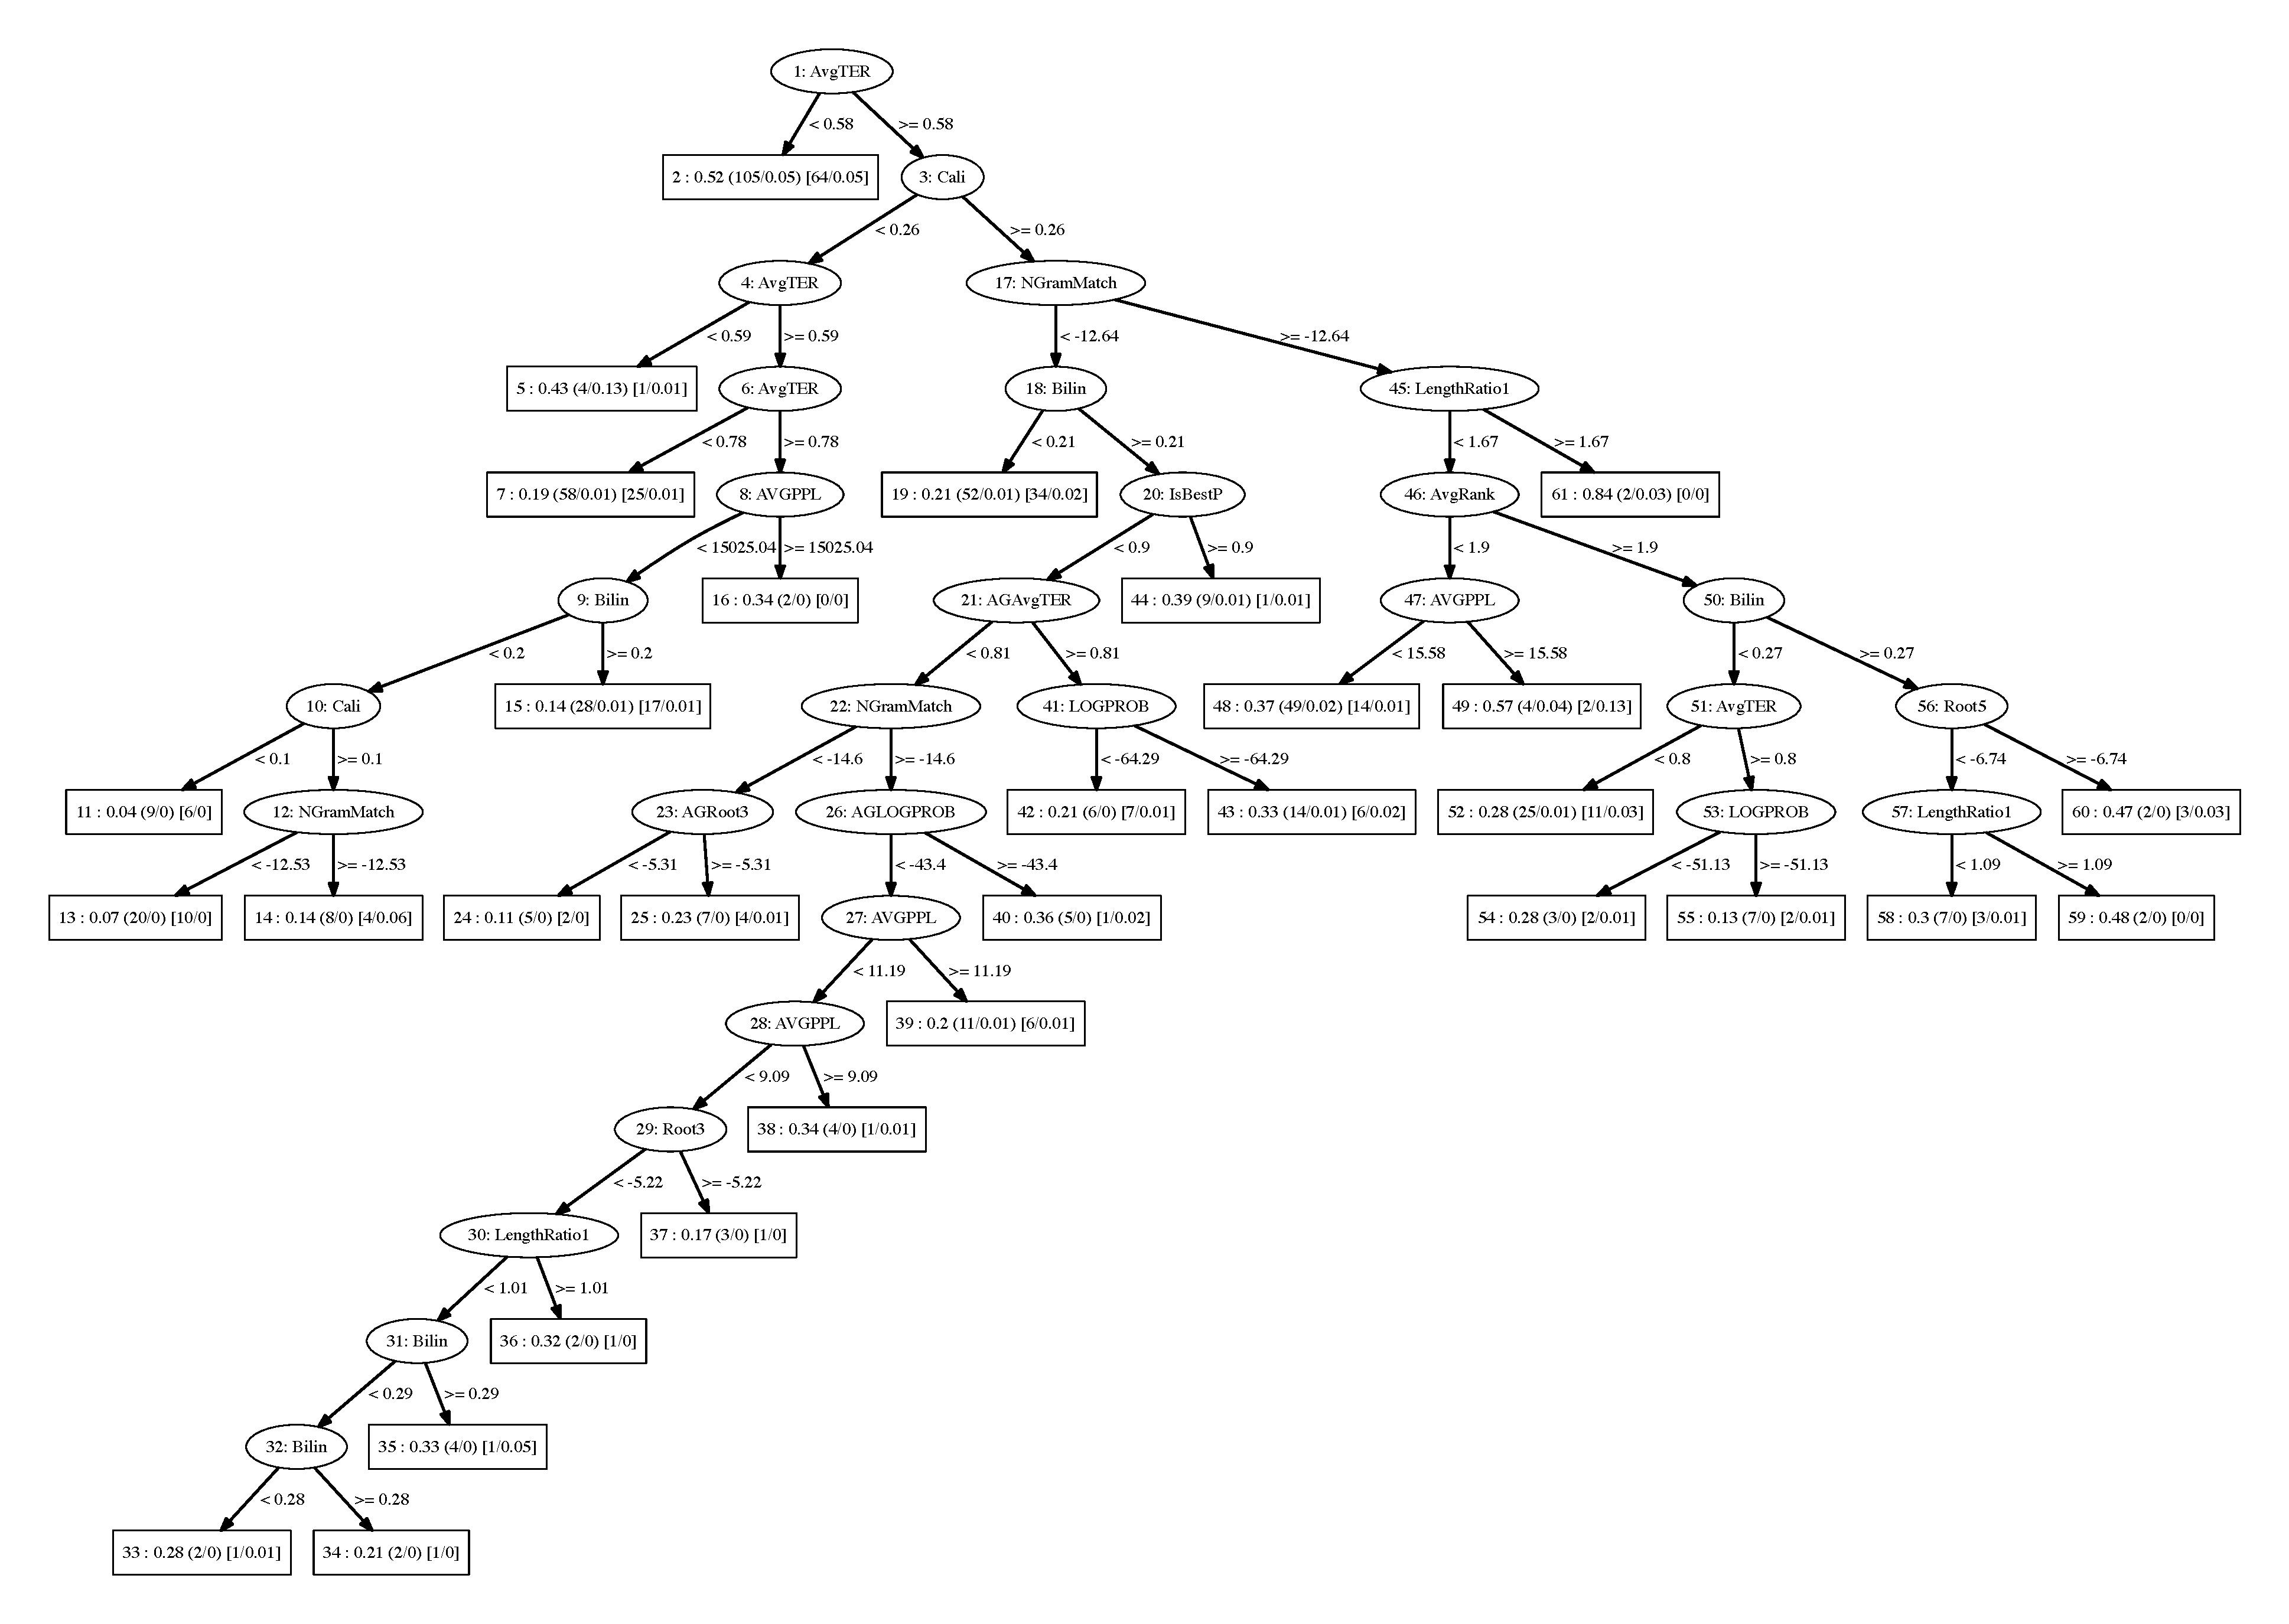
\includegraphics[width=\textwidth]{DT/example.pdf}
  \caption{The visualization for the Decision Tree Model.
}
    \label{dtexample}
\end{figure}

\subsection{Linear Regression}
\begin{table}[h]
\center
\begin{tabular}{c|c}
\hline
Feature Set           & BLEU Score \\ \hhline{==}
(S)entence features   & 37.84      \\ \hline
(W)orker features     & 36.92     \\ \hline
(R)anking features    & 35.69     \\ \hline
(C)alibration feature & 38.27      \\ \hline
S+W+R features        & 38.69     \\ \hline
S+W+R+B features      & 39.23    \\ \hline
All features          & 39.80     \\ \hline
\end{tabular}
\caption{The translation quality for Linear Regression}
\label{lrbleu}
\end{table}

\section{Quality Control Analysis}
Compared to the baseline method, the MERT model, Decision Tree Model and Linear Regression Model all achieve much better performance, which means.







